
\subsubsection{UC1 - Visualizzazione guida introduttiva}
\begin{itemize}
	\item \textbf{Attori Primari}: utente generico;
	\item \textbf{Descrizione}: l'utente visualizza una guida riguardante l'installazione ed il funzionamento del plug-in Metamask\glo. Tale guida ha il compito di spiegare come impostare le chiavi del plug-in e come utilizzarlo per accedere al sistema;
	\item \textbf{Scenario principale}: l'utente accede alla pagina introduttiva del sito web e visualizza la guida;
	\item \textbf{Precondizione}: il sistema è raggiungibile e funzionante, l'utente accede alla pagina iniziale del sito della piattaforma;
	\item \textbf{Postcondizione}: il sistema fornisce all'utente, attraverso la lettura della guida, tutte le istruzioni necessarie alla registrazione ed all'autenticazione.
	
	
\end{itemize}
\subsubsection{UC2 - Registrazione}
\begin{figure}[h]
	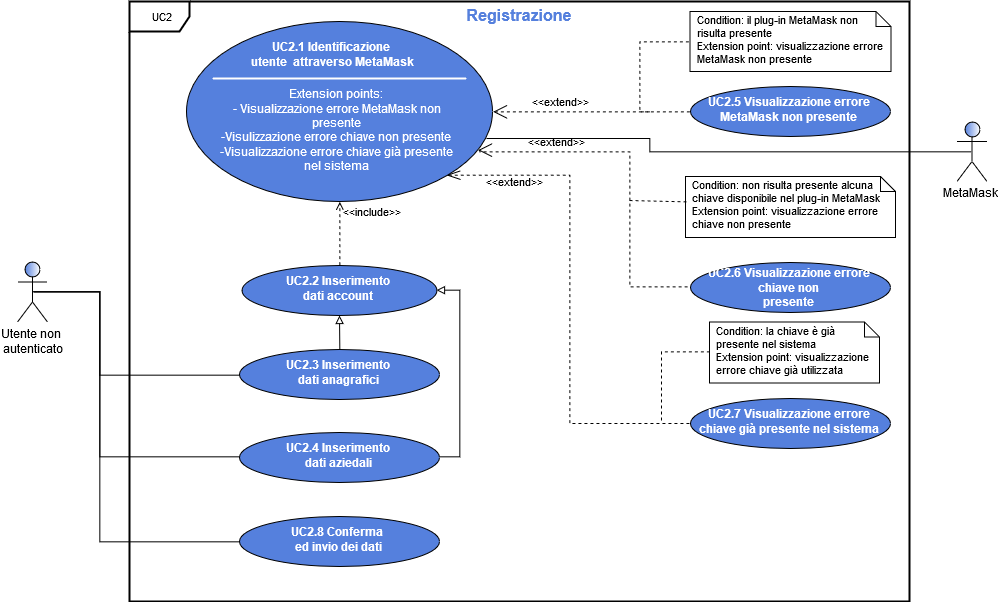
\includegraphics[width=16cm]{res/images/UC2Registrazione.png}
	\centering
	\caption{UC2 - Registrazione}
\end{figure}
\begin{itemize}
	\item \textbf{Attori Primari}: utente non autenticato;
	\item \textbf{Attori Secondari}: MetaMask\glo;
	\item \textbf{Descrizione}: per effettuare il procedimento di registrazione, l'utente deve disporre di una chiave\glosp non ancora utilizzata per la registrazione all'interno del sistema, e deve compilare tutti i campi necessari;
	\item \textbf{Scenario principale}: 
		il sistema controlla la presenza di MetaMask\glosp e verifica che la prima chiave\glosp in esso contenuta non sia già associata ad un utente registrato alla piattaforma. Successivamente rende disponibili i campi da compilare per la registrazione. Dunque, se:
	\begin{enumerate}[label=\alph*.]
	
		\item l'utente vuole registrarsi come normale \textbf{cittadino}: 
		\begin{enumerate}[label=\roman*.]
			\item l'utente inserisce i dati anagrafici [UC2.3];
			\item l'utente conferma ed invia i dati inseriti [UC2.8].
		\end{enumerate}
		
		
		\item l'utente vuole registrare la propria \textbf{azienda}:
		\begin{enumerate}[label=\roman*.]
			\item l'utente inserisce i dati aziendali [UC2.4];
			\item l'utente conferma ed invia i dati inseriti [UC2.8].
		\end{enumerate}
		
		
		
	\end{enumerate}
	\item \textbf{Precondizione}: l'utente ha MetaMask\glosp installato e correttamente impostato sul proprio browser, viene considerato dal sistema come un utente non autenticato. La prima chiave\glosp nel plug-in non risulta già associata ad alcun account nel sistema. L'utente intende registrarsi come cittadino o registrare la propria azienda; 
	\item \textbf{Postcondizione}: l'utente è registrato correttamente nel sistema come cittadino o azienda.
	
\end{itemize}
\subsubsection{UC2.1 - Identificazione utente attraverso MetaMask}
\begin{itemize}
	\item \textbf{Attori Primari}: utente non autenticato;
	\item \textbf{Attori Secondari}: MetaMask\glo;
	\item \textbf{Descrizione}: il sistema verifica la presenza del plug-in MetaMask\glo, al quale richiede la chiave\glosp che l'utente desidera usare come identificativo e metodo di pagamento. Essendo la chiave\glosp univoca, il sistema controlla che nessun utente registrato stia attualmente utilizzandola. Il sistema mostra infine l'interfaccia contenente il form di registrazione;
	\item \textbf{Scenario principale}: il sistema, prima di mostrare il form per la registrazione, controlla che la chiave di riferimento individuata dal plug-in MetaMask\glosp non sia associata ad alcun utente registrato al sistema;
	\item \textbf{Estensioni}:
	\begin{itemize}
		\item \textbf{UC2.5}: se il plug-in MetaMask\glosp non risulta installato nel browser dell'utente, o è stato disabilitato, esso viene avvisato tramite l'apposito messaggio di errore;
		\item \textbf{UC2.6}: se l'utente non possiede una chiave\glosp su MetaMask\glo, esso viene avvisato tramite l'apposito messaggio di errore;
		\item \textbf{UC2.7}: se è presente una chiave su MetaMask\glo, ma il sistema rileva che essa è già stata utilizzata per la registrazione sulla piattaforma, allora l'utente viene avvisato attraverso l'apposito messaggio di errore.
	\end{itemize}
	\item \textbf{Precondizione}: l'utente ha inserito i propri dati per registrarsi nel sistema;
	\item \textbf{Postcondizione}: il sistema ha verificato che la chiave\glosp con la quale l'utente sta cercando di registrarsi non risulti già utilizzata nel sistema. La chiave è salvata e verrà utilizzata durante la registrazione. All'utente è permesso compilare i dati relativi alla tipologia di registrazione richiesta.
	
\end{itemize}
\subsubsection{UC2.2 - Inserimento dati account}
\begin{figure}[h]
	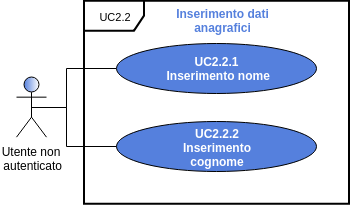
\includegraphics[width=8cm]{res/images/UC2-2RegistrazioneGenerale.png}
	\centering
	\caption{UC2.2 - Inserimento dati account}
\end{figure}
\begin{itemize}
	\item \textbf{Attori Primari}: utente non autenticato;
	\item \textbf{Descrizione}: l'utente compila il form contenente i dati relativi all'account, campi richiesti sia nella registrazione di un cittadino che in quella di un'azienda;
	\item \textbf{Scenario principale}: l'utente compila tutti i campi del form riguardanti l'account, ovvero:
	\begin{enumerate}[label=\alph*.]
		\item l'utente inserisce l'email da associare all'account [UC2.2.1];
		\item l'utente inserisce l'indirizzo di residenza (sede nel caso della registrazione di un'azienda) da associare all'account [UC2.2.2];
	\end{enumerate}
	\item \textbf{Specializzazione}:
	\begin{itemize}
		\item \textbf{UC2.3}: l'utente inserisce i dati relativi alla registrazione di un cittadino;
		\item \textbf{UC2.4}: l'utente inserisce i dati relativi alla registrazione di un'azienda.
		
	\end{itemize}
	\item \textbf{Precondizione}: l'utente è entrato nel form per eseguire la procedura di registrazione. Il sistema ha rilevato e salvato una chiave\glosp valida (non associata ad alcun utente registrato alla piattaforma) attraverso il plug-in MetaMask\glo;
	\item \textbf{Postcondizione}: l'utente ha compilato i campi relativi ai dati dell'account richiesti da ogni tipologia di registrazione.
	
\end{itemize}
\subsubsection{UC2.2.1 - Inserimento e-mail}
\begin{itemize}
	\item \textbf{Attori Primari}: utente non autenticato;
	\item \textbf{Descrizione}: al fine di portare a termine il processo di registrazione l'utente deve inserire un indirizzo e-mail, campo ritenuto obbligatorio;
	\item \textbf{Scenario principale}: l'utente compila il campo relativo all'indirizzo e-mail;
	\item \textbf{Precondizione}: il sistema ha reso disponibile il campo per l'inserimento dell'indirizzo e-mail;
	\item \textbf{Postcondizione}: l'utente ha compilato il campo con la propria e-mail.
	
\end{itemize}
\subsubsection{UC2.2.2 - Inserimento indirizzo di residenza}
\begin{itemize}
	\item \textbf{Attori Primari}: utente non autenticato;
	\item \textbf{Descrizione}: al fine di portare a termine il processo di registrazione l'utente deve inserire un indirizzo di residenza, campo ritenuto obbligatorio. Esso è composto da: 
	\begin{itemize}
	\item nome della via e numero civico;
	\item paese;
	\item provincia;
	\item CAP.

	\end{itemize}
	\item \textbf{Scenario principale}: l'utente compila il campo relativo all'indirizzo di residenza;
	\item \textbf{Precondizione}: il sistema ha reso disponibile i campi per l'inserimento dell'indirizzo di residenza;
	\item \textbf{Postcondizione}: l'utente ha compilato il campo con l'indirizzo relativo alla residenza.
\end{itemize}
\subsubsection{UC2.3 - Inserimento dati anagrafici}
\begin{figure}[h]
	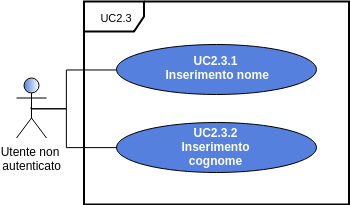
\includegraphics[width=5cm]{res/images/UC2-3Registrazione-cliente.png}
	\centering
	\caption{UC2.3 - Inserimento dati anagrafici}
\end{figure}
\begin{itemize}
	\item \textbf{Attori Primari}: utente non autenticato;
	\item \textbf{Descrizione}: l'utente compila i campi relativi alla registrazione alla piattaforma come cittadino;
	\item \textbf{Scenario principale}: l'utente ha cliccato sul pulsante relativo alla registrazione come cittadino, il sistema rende disponibile il form di registrazione relativo e l'utente compila tutti i campi necessari. In particolare, oltre ai dati account:
	\begin{enumerate}[label=\alph*.]
		\item l'utente inserisce il proprio nome [UC2.3.1];
		\item l'utente inserisce il proprio cognome [UC2.3.2].
	\end{enumerate}
	\item \textbf{Precondizione}: l'utente ha cliccato sul pulsante relativo alla registrazione come cittadino, il sistema rende disponibile il form di registrazione. Il sistema ha rilevato e salvato una chiave\glosp valida attraverso MetaMask\glo;
	\item \textbf{Postcondizione}: l'utente ha compilato i campi relativi alla registrazione di un cittadino alla piattaforma.
\end{itemize}
\subsubsection{UC2.3.1 - Inserimento nome}
\begin{itemize}
	\item \textbf{Attori Primari}: utente non autenticato;
	\item \textbf{Descrizione}: al fine di portare a termine il processo di registrazione di un nuovo cittadino, l'utente deve inserire il proprio nome, campo ritenuto obbligatorio;
	\item \textbf{Scenario principale}: l'utente compila il campo relativo al nome;
	\item \textbf{Precondizione}: il sistema ha reso disponibile il campo per l'inserimento del nome;
	\item \textbf{Postcondizione}: l'utente ha compilato il campo con il proprio nome.
\end{itemize}
\subsubsection{UC2.3.2 - Inserimento cognome}
\begin{itemize}
	\item \textbf{Attori Primari}: utente non autenticato;
	\item \textbf{Descrizione}: al fine di portare a termine il processo di registrazione di un nuovo cittadino, l'utente deve inserire il proprio cognome, campo ritenuto obbligatorio;
	\item \textbf{Scenario principale}: l'utente compila il campo relativo al cognome;
	\item \textbf{Precondizione}: il sistema ha reso disponibile il campo per l'inserimento del cognome;
	\item \textbf{Postcondizione}: l'utente ha compilato il campo con il proprio cognome.
\end{itemize}

\subsubsection{UC2.4 - Inserimento dati aziendali}
\begin{figure}[h]
	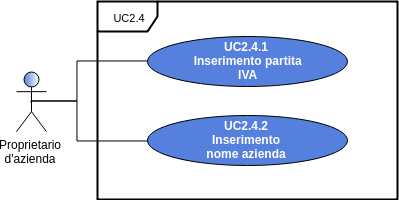
\includegraphics[width=6cm]{res/images/UC2-4RegistrazioneAzienda.png}
	\centering
	\caption{UC2 - Inserimento dati aziendali}
\end{figure}
\begin{itemize}
	\item \textbf{Attori Primari}: proprietario d'azienda;
	\item \textbf{Descrizione}: l'utente compila i campi relativi alla registrazione della propria azienda sulla piattaforma;
	\item \textbf{Scenario principale}: l'utente ha cliccato sul pulsante di registrazione di un'azienda, il sistema rende disponibile il form di registrazione relativo e l'utente compila tutti i campi necessari. In particolare, oltre ai dati account:
	\begin{enumerate}[label=\alph*.]
		\item l'utente inserisce la partita IVA dell'azienda [UC2.4.1];
		\item l'utente inserisce il nome dell'azienda [UC2.3.2].
	\end{enumerate}
	\item \textbf{Precondizione}: l'utente ha cliccato il link per la registrazione di un'azienda. Il sistema ha rilevato e salvato una chiave\glosp valida (non associata ad alcun utente registrato alla piattaforma) attraverso MetaMask\glo;
	\item \textbf{Postcondizione}: l'utente ha compilato i campi relativi alla registrazione di un'azienda alla piattaforma.
\end{itemize}
\subsubsection{UC2.4.1 - Inserimento partita IVA}
\begin{itemize}
	\item \textbf{Attori Primari}: proprietario d'azienda;
	\item \textbf{Descrizione}: al fine di portare a termine il processo di registrazione della propria azienda, l'utente deve inserire la relativa partita IVA, campo ritenuto obbligatorio;
	\item \textbf{Scenario principale}: l'utente compila il campo relativo alla partita IVA;
	\item \textbf{Precondizione}: il sistema ha reso disponibile il campo per l'inserimento della partita IVA;
	\item \textbf{Postcondizione}: l'utente ha compilato il campo con la partita IVA dell'azienda che intende registrare.
\end{itemize}
\subsubsection{UC2.4.2 - Inserimento nome azienda}
\begin{itemize}
	\item \textbf{Attori Primari}: proprietario d'azienda;
	\item \textbf{Descrizione}: al fine di portare a termine il processo di registrazione della propria azienda, l'utente deve inserire il relativo nome aziendale, inteso come ragione sociale, campo ritenuto obbligatorio;
	\item \textbf{Scenario principale}: l'utente compila il campo relativo al nome aziendale;
	\item \textbf{Precondizione}: il sistema ha reso disponibile il campo per l'inserimento del nome aziendale;
	\item \textbf{Postcondizione}: l'utente ha compilato il campo con il nome dell'azienda che intende registrare.
\end{itemize}

\subsubsection{UC2.5 - Conferma ed invio dei dati}
\begin{itemize}
	\item \textbf{Attori Primari}: utente non autenticato;
	\item \textbf{Descrizione}:
	l'utente preme il pulsante per la conferma e l'invio dei dati. A schermo viene mostrato un messaggio che conferma il successo dell'operazione;
	\item \textbf{Scenario principale}: l'utente preme il pulsante di verifica ed invio dei dati dopo aver compilato i campi del form;
	\item \textbf{Precondizione}: il sistema permette all'utente di compilare il form di registrazione. \`E presente il pulsante per la conferma dei dati;
	\item \textbf{Postcondizione}: viene visualizzato un messaggio per informare l'utente del fatto che la richiesta di registrazione è avvenuta con successo.
\end{itemize}

\subsubsection{UC3 - Visualizzazione errore MetaMask\glosp non presente}
\begin{itemize}
	\item \textbf{Attori Primari}: utente non autenticato;
	\item \textbf{Descrizione}: l'utente visualizza un errore relativo al fatto che MetaMask\glosp non risulta installato o attualmente disabilitato;
	\item \textbf{Scenario principale}: l'utente non ancora identificato dal sistema tenta di accedere a sezioni che necessitano la presenza di MetaMask\glosp, e quest'ultimo non è installato o attualmente disabilitato;
	\item \textbf{Precondizione}: MetaMask\glosp non è presente nel browser dell'utente o è attualmente disabilitato;
	\item \textbf{Postcondizione}: viene visualizzato un messaggio d'errore per informare l'utente del fatto che è necessario installare ed abilitare MetaMask\glosp per proseguire.
	
\end{itemize}

\subsubsection{UC4 - Visualizzazione errore chiave non 
	presente}
\begin{itemize}
	\item \textbf{Attori Primari}: utente non autenticato;
	\item \textbf{Attori Secondari}: MetaMask\glo;
	\item \textbf{Descrizione}:
	l'utente visualizza un messaggio di errore relativo al fatto che non è stata rilevata nessuna chiave\glosp all'interno del plug-in MetaMask\glo;
	\item \textbf{Scenario principale}: l'utente tenta di accedere ad una sezione del sito che necessita l'identificazione di una chiave\glosp attraverso MetaMask\glo, e questo non contiene almeno una chiave\glo;
	\item \textbf{Precondizione}: il plug-in MetaMask\glosp è correttamente configurato, ma non è presente nessuna chiave\glo;
	\item \textbf{Postcondizione}: viene visualizzato un messaggio d'errore per informare l'utente del fatto che in MetaMask\glosp non è stata rilevata alcuna chiave\glo.
	
\end{itemize}

\subsubsection{UC5 - Visualizzazione errore chiave già presente nel sistema}
\begin{itemize}
	\item \textbf{Attori Primari}: utente non autenticato;
	\item \textbf{Attori Secondari}: MetaMask\glo;
	\item \textbf{Descrizione}:
	l'utente visualizza un messaggio di errore relativo al fatto che la chiave\glosp reperita da MetaMask\glosp risulta già presente nella piattaforma;
	\item \textbf{Scenario principale}: l'utente tenta di registrarsi al sito utilizzando una chiave\glosp già presente nel sistema;
	\item \textbf{Precondizione}: MetaMask\glosp è correttamente configurato, ma la chiave\glosp selezionata nel plug-in è già stata utilizzata nella piattaforma per registrare un utente;
	\item \textbf{Postcondizione}: viene visualizzato un messaggio d'errore per informare l'utente del fatto che la chiave\glosp selezionata MetaMask\glosp è già stata utilizzata nella piattaforma per la registrazione di un altro utente, e quindi che necessita di un'altra chiave per effettuare una nuova registrazione.
\end{itemize}

